\chapter{Contraction Hierarchies}\label{chapter:ch}

\todo{Historie und Zitieren}

\begin{definition}[Upward Graph]
    Sei $G = (V, E)$ und ${vtl} \coloneq V \to \mathbb{N}$ die injektive \emph{vertex-to-level} Funktion. Dann ist $G_u = (V, E_u)$ ein \emph{upward Graph} zu $G$ wenn gilt:
    \begin{enumerate}
        \item\label{ch:definition:legal_edges}
        $E_u$ enthält nur Kanten $(t, h, w)$ mit $t, h \in V$ und $w \in \mathbb{N}$ für die ${vtl}(t) < {vtl}(h)$ und $w >= {spd}_{G}((t, h))$ gilt.

        \item\label{ch:definition:upward}
        $E_u$ enthält mindestens alle Kanten $(t, h, {spd}_{G}((t, h)))$ mit $t, h \in V$, für die gilt, dass $h$ das größte und $t$ das zweitgrößte Level auf dem kürzesten Weg auf $G$ von $t$ nach $h$ hat.
    \end{enumerate}
\end{definition}

Der Name des upward Graphen ergibt sich daher, dass die Suche in einem upward Graph auf das Level bezogen nur \emph{aufwärts} geht.

\begin{figure}
    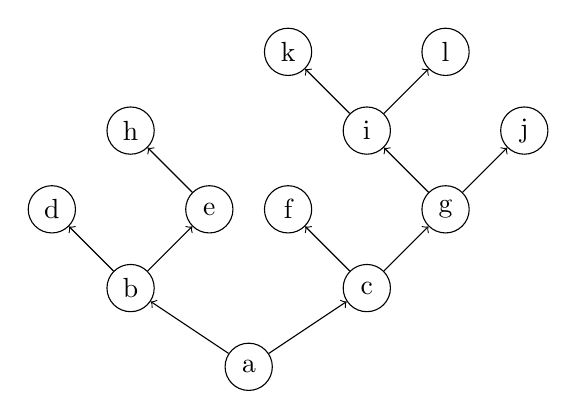
\begin{tikzpicture}
        % Nodes
        \node[circle, draw, minimum size=0.6cm, inner sep=0pt] at (2.5, 0)  (a)    {a};
        \node[circle, draw, minimum size=0.6cm, inner sep=0pt] at (1, 1)  (b)    {b};
        \node[circle, draw, minimum size=0.6cm, inner sep=0pt] at (4, 1)  (c)    {c};
        \node[circle, draw, minimum size=0.6cm, inner sep=0pt] at (0, 2)  (d)    {d};
        \node[circle, draw, minimum size=0.6cm, inner sep=0pt] at (2, 2)  (e)    {e};
        \node[circle, draw, minimum size=0.6cm, inner sep=0pt] at (3, 2)  (f)    {f};
        \node[circle, draw, minimum size=0.6cm, inner sep=0pt] at (5, 2)  (g)    {g};
        \node[circle, draw, minimum size=0.6cm, inner sep=0pt] at (1, 3)  (h)    {h};
        \node[circle, draw, minimum size=0.6cm, inner sep=0pt] at (4, 3)  (i)    {i};
        \node[circle, draw, minimum size=0.6cm, inner sep=0pt] at (6, 3)  (j)    {j};
        \node[circle, draw, minimum size=0.6cm, inner sep=0pt] at (3, 4)  (k)    {k};
        \node[circle, draw, minimum size=0.6cm, inner sep=0pt] at (5, 4)  (l)    {l};


        \draw[->]  (a) -- (b);
        \draw[->]  (a) -- (c);

        \draw[->]  (b) -- (d);
        \draw[->]  (b) -- (e);

        \draw[->]  (c) -- (f);
        \draw[->]  (c) -- (g);

        \draw[->]  (e) -- (h);

        \draw[->]  (g) -- (i);
        \draw[->]  (g) -- (j);

        \draw[->]  (i) -- (k);
        \draw[->]  (i) -- (l);
    \end{tikzpicture}
\end{figure}


Aus dieser Definition folgt, dass der kürzeste Pfad zwischen zwei Knoten in $G_u$ ist also mindestens genausolang ist wie in $G$.
% https://cstheory.stackexchange.com/questions/23767/why-is-label-pruning-possible-with-hub-labeling

\todo{Zeiche zwei Suchbäume, jeweils in G und Gu}

\begin{definition}[Downward Graph]
    Sei $G = (V, E)$ und ${vtl} \coloneq V \to \mathbb{N}$ die injektive \emph{vertex-to-level} Funktion. Dann ist ein upward Graph des Umkehrgraphens $G^T$ ein \emph{downward Graph} zu $G$.
\end{definition}


Ein \emph{Contracted Graph} ist die Datenstruktur, mit deren Hilfe schnell kürzeste Wege gefunden werden können.
Bevor im Folgenden verschiedene Arten beschrieben werden, wie, ein Contracted Graph erstellt werden kann, wird eine allgemeingültige Definition eingeführt.



Die Suche eines kürzesten Pfades von $u$ nach $v$ auf einem Contracted Graph gestaltet sich nun wie folgt:
Auf $G_u$ wird eine Breitensuche von $u$ und auf $G_d$ eine Breitensuche von $v$ durchgeführt.
\autoref{fig:ch:beispiel_suche} zeigt das auf- und absteigen der Level an einem Beispiel.

Gibt es einen Pfad von $u$ nach $v$, so werden beide Suchen den Knoten $t$ mit dem höchsten Level auf dem kürzesten Pfad finden.
Die kürzeste Pfad Distanz ist dann die Summe der Distanz der upward Suche ($u \to t$) und der downward Suche ($v \to t$).
Der kürzeste Pfad ist der setzt sich aus den beiden Pfaden der upward und downward Suche zusammen, wobei der in beiden Teilen vorkommenden Knoten $t$ in einem Teil entfernt und werden muss.
Da $G_d$ den Pfad von $v$ nach $t$ findet, muss dieser Teil des Pfades invertiert werden, bevor die Teilpfade konkatiniert werden.

\begin{figure}[ht]
    \centering
    \begin{tikzpicture}
        \node[circle, draw] at (0 * 1.5, -5 * 0.75)  (a)    {u};
        \node[circle, draw] at (1 * 1.5, -7 * 0.75)  (b)    {b};
        \node[circle, draw] at (2 * 1.5, -6 * 0.75)  (c)    {c};
        \node[circle, draw] at (3 * 1.5, -1 * 0.75)  (d)    {d};
        \node[circle, draw] at (4 * 1.5, -0 * 0.75)  (e)    {t};
        \node[circle, draw] at (5 * 1.5, -3 * 0.75)  (f)    {f};
        \node[circle, draw] at (6 * 1.5, -2 * 0.75)  (g)    {g};
        \node[circle, draw] at (7 * 1.5, -4 * 0.75)  (h)    {v};

        % draw axis
        \draw[->] (-1, -7 * 0.75) -- (-1, 0) node[above] {Level};

        \draw[->]  (a) -- (d);
        \draw[->]  (d) -- (e);
        \draw[->]  (h) -- (g);
        \draw[->]  (g) -- (e);

        \draw[->, dotted]  (a) -- (b);
        \draw[->, dotted]  (b) -- (c);
        \draw[->, dotted]  (c) -- (d);
        \draw[->, dotted]  (g) -- (f);
        \draw[->, dotted]  (f) -- (e);

    \end{tikzpicture}
    \caption{Beispiel einer Suche in einem Contrated Graph}
    \label{fig:ch:beispiel_suche}
\end{figure}

\begin{beweis}
    Der Beweis der Korrektheit folgt in zwei Schritte.

    \begin{enumerate}
        \item
              Es existiert ein kürzester Pfad von $u$ nach $v$ in $G$ $\Rightarrow$ Er wird in $C$ gefunden.

              Da ${vtl}$ injektiv ist, existiert genau ein Knoten $t$ mit dem höchstem Level. Zerscheide den Pfad $(u, \dotsc, v)$ in zwei Teile:  und $(u, \dotsc, t)$ und $(t, \dotsc, v)$. Die Tupel benachbarten Knoten in $(u, \dotsc, t)$ sind nach \autoref{ch:definition:downward} der Definition des upward Graph Kanten von $G_u$. Daher wird $t$ im upward Graph gefunden. Analog dazu wird $t$ in $G_d$ gefunden, die Tupel benachbarter Knoten im Pfad $(t, \dotsc, v)$ sind nach \autoref{ch:definition:upward} der Definition des downward Graphs Kanten von $G_d$.

              Da die Tupel Kanten der Graphen sind, findet eine Breitensuche sie.

        \item
              Es existiert kein kürzester Pfad von $u$ nach $v$ in $G$ $\Rightarrow$ Es wird in $C$ kein Pfad gefunden gefunden.

              Angenommen, es würde ein Pfad in C gefunden werden. Die Tupel benachbarter Knoten des Pfades müssten dann Kanten in C sein.
              Mindestens einer diese Kanten hätte dann ein Gewicht welches gegen \autoref{ch:definition:legal_edges} der Definition verstoßt.
    \end{enumerate}

    Daher gilt, die Suche der kürzesten Pfad Distanz in $C$ ist äquivalent zu der in $G$
\end{beweis}

\section{Erstellung}

Das Ziel der Contraction Hierarchies ist es aus dem Graph zwei Teilgraphe mit Abkürzungen (\emph{shortcuts}) zu erstellen.
Auf diesen Graphen kann mit einer Breitensuche effizient ein Knoten gefunden werden, der auf dem kürzesten Pfad zwischen zwei Knoten liegt.

\subsection{Contraction}


\subsubsection{Bottom-Up}


\clearpage

\todo{überhaupt Möglich weil sum degree**2 zu hoch?}

Für die triangulierten Graphen ist es möglich den klassischen Contraction Hierarchie Algorithmus mit der Knoten-Differenz und Lazy-poping (\cite{geisberger2008contraction}) anzuwenden, wobei auch ein signifikanter Speedup erzielt werden kann. \todo{Tabelle Speedup}
Darauf aufbauend kann auch ein Hub Labeling erstellt werden, wodurch nochmals ein signifikanter Speedup erzielt werden kann.
Für die Sichtbarkeitsgraphen gilt dies jedoch nicht, auf den verwendeten Computern konnte für keinen von ihnen innerhalb von drei Tagen eine Erstellung abgeschlossen werden.
\todo{Wie weit sind sie gekommen? Was ist der größtmögliche Graph, für den dies möglich ist?}
Der Grund hierfür ist naheliegend: Der Algorithmus führt für jeden In-Nachbar eine one-to-many Suche zu allen Out-Nachbarn aus.
Die Durschnitliche Suchtiefe ist dabei sehr hoch, da Knoten des Sichtbarkeitsgraphen mit einer hohen Wahrscheinlichkeit eine Kanten mit großem Gewicht haben, die zum Beispiel über einen Ozean auf die am weitest entfernte Küste zeigt.
Das begrenzen der Suche auf wenige Hops ist dabei auch nicht hilfreich, da die Durschnitliche Hop-Länge von kürzesten Pfaden auf Sichtbarkeitsgraph gering ist eine so begrenzte Suche also viele kürzeste Pfade nicht finden würde.

Daher müssen für die Sichtbarkeitsgraphen andere Methoden gefunden werden.
Die naheliegendste Idee ist das direkte Berechnen der CH Edges und HL Labels.
Dies ist zwar sehr rechenintensiv, es muss für jeden Knoten eine one-to-many bzw. one-to-all Suche durchgeführt werden, dies ist jedoch schneller möglich, also für jeden in-Nachbar eine one-to-many Suche zu berechnen.



Wir erstellen zwei neue Graphen aus einem input Graphen.

Upward Graph: (u, v) ist Kante wenn der V des höchsten Leven auf dem kürzstem Pfad von u nach v hat und u den zweithöchsten.

Downward Graph: (u, v) ist in Kante wenn v den höchsten Level auf dem Kürzsten Pfad von v nach u hat und u den zweithöchsten.
TODO ist das so richtig?

Wenn Graph bidirectional ist, dann upward graph == downard graph

((u, v), s) ist jeweils ein shortcut, wenn der kürzste Pfand länger als 2 Hops ist.

Die Auswahl von S ist nicht genau definiert, jedoch muss es am Ende möglich sein die Shortcuts auszupacken.
Bei single step contraction verstehe ich das, bei brute Force ist mir das aber noch nicht ganz klar. Reicht 1 HashMap dann oder brauche ich jeweils für eine für Up and Downward Graph.


Diese Defintion ist ein bisschen anders als vielleicht anders gesehen. Häufig? wird auf dem Downward Graph eine Rückwärtssuche gemacht. Ich möchte aber keine extra Suche und so dafür implementieren, daher ist der Downward graph auch ein Out Graph.

Datenstruktur ähnlich zu Reversible Graph. Da einmal fester Graph nicht mehr verändert wird nutze ich einen VecGraph wobei die Edges nach Level Tail geordnet sind.

\section{Query}
Auf jedem kürsten Pfad gibt es einen Vertex mit höchstem Level. Die Suchen auf dem upward und downard graph treffen sich in diesem.

Bild Zicksack. Mit Shortcuts

Early stop nicht trivial möglich TODO WARUM (Es gab auf Stackoverflow mal ein Gegenbeispiel aber ich finde es nicht mehr :( Der CH Graph ist garantiert ein Shortest Path Tree (Bei Bruteforce aber schon, daher kein Stall notwendig??? TODO))

Warum schnell? Wir betrachten nur einen Teil der Vertices, die haben dafür aber garantiert? mehr Nachbarn. Trotzdem Tradeofff? Immer?

\subsection{Heuristic}

Ist es möglich, bzw lohnt es sich Heuristic zu verwenden? Lowerbound für Zielfindung oder Upperbound welche nicht verwendet werden müssen?


\section{Single Step contraction}
Zuerst normalen Vorgang erklären. Dann sind die Wörter, die später benutzt werden bereits definiert.

Contraction Heuristiken

Wir betrachten Vertex v. tail -> v -> head.
Füge shortcut tail -> head ein, wenn tail -> v -> head der einzigste kürzste Weg ist.
Dafür eine one to many without v Vorwärtssuche.
shortcut wenn shortcut cost < dijkstra cost
without kann deutlich teuerer machen (TODO Beweis).

daher besser ohne without. Dann aber shortcut wenn cost <= dijkstra cost.
Die Ungleichung wird also abgeschwächt.
Zusätzlich kann man noch max\_hops anschauen, aber das ist für die Visibility Graphen nur bedingt sinvoll, da kürzste wege nur wenig hops. TODO Beweis

Heuristic.
Statt suche kann man auch heursitc benutzten.
shortcut distance < dijksta cost ==> shortcut distance <= upper bound
also shortcut distance <= upper bound => füge shortcut ein

Used heuristics:
TrivialeHeuristic (all in). Füge jeden shortcut ein.

Landmarks. Gut für größere Entfernungen.
Es reicht zu zeigen, dass shortcut distance > upperbound für ein Landmark ist. Dann bereits kein shortcut.
Viele Landmakrs, weniger shortcuts, mehr checks (vielleicht gibt es Break-Even point?). Wenige Landmarks, mehr shortcuts, weniger checks?
TODO Vielleicht noch check einbauen dass wenn shortcut distance == lower bound, dann shortcut zwingen notwendig ist.
TODO Wenn shortcut distance == lowerbound(head) - lowerbound(tail) dann checken ob tail auf landmark path (head). Oder ist das unnötig nach oben?

CH / HL als Heuristic.
Dann ist lowerbound == upperbound und damit wie dijkstra ohne without. Kann sich unter umständen lohnen.


single step contraction?? TODO name

\subsection{Bottum-Up}

Greddy lazy poping vs neighbor update.

lazy poping für vis graphen nicht sinvoll?

Neighbor update für vis graphen nicht sinvoll?
Vielleicht nur updaten, nachdem n nachbarn contracted worden?

Vielleicht nur n mal insgesammt updaten? alle 10\% neu berechnen?



Heuristic egde difference (zufall)
Vis graphen haben sehr hohen degree (TODO Beweis).
Daher degree x degree viele checks, das gehtn schnell in die Millionen bis Milliarden.
Idee: betrachte nur ein Subset (tails, heads) und schaue ob und wie genau dieses die Edge difference aproximiert.

Das kann dann wieder für andere Methoden benutzt werden.

Plot hitting set vs bottom-up order


\subsection{Top-Down}



\section{Hitting Set Berechnung}
Vorraussetzung für das Bruteforcing ist eine Funktion $f \coloneq V \to \mathbb{N}$, welche den Knoten einem \emph{Level}

Level-to-vertex

TODO Edge difference factor
überlegung ist, nur wenige hops. Daher reicht es eigenbtlich direkte Nachbarn anschauen.

Hitting set
Berechne Hitting Set mit Dijkstra oder CH, HL aus vorheriger Runde.
TODO Qualität des Hitting Set durch aproximitation der HL Size.

Bottum up contraction auf graph, verwende dieses für Vis Graph.
TODO

Random


\section{Brute force}

Berechne die Kanten stupide nach Defintion. Hoffnung: Suche ist relativ lokal? TODO Beweis? Avg dijksta rang?

Das mit den Shortcuts ist dann nicht so einfach. TODO Bild

